\chapter{Einleitung}
Quantenstrukturen, wie sie heutzutage hergestellt werden können, eröffnen neue Möglichkeiten im Bereich der ultraschnellen Elektronik und Photonik. Solche Strukturen lassen sich in aller Regel als \emph{offene} Systeme beschreiben. Es findet ein Austausch von lokal erhaltenen Fermionen -- die Erhaltung wird durch eine lokale Kontinuitätsgleichung beschrieben -- mit der Umgebung statt. Die Umgebung besteht dabei aus mindestens zwei verschiedenen Teilchen-Reservoirs. In diesem Fall kann also ein Nicht-Gleichgewichtszustand erreicht werden, beispielsweise durch das Anlegen einer Spannung. Das zu untersuchende System besitzt eine endliche Ausdehnung im Raum. Es muss im Nicht-Gleichgewichtsfall folglich ein Strom durch die Oberfläche als Rand des Systems fließen. Wir beschränken uns hier auf eindimensionale Quantenstrukturen, für die also die interessante Physik in einer Dimension stattfindet. Dabei wollen wir den Strom der Teilchen, also den quantenmechanischen Transport beschreiben. Dies geschieht allgemein in verschiedenen Anwendungsfällen (Hydrodynamik, Aerodynamik, Elektronik, Neutronentransport, \dots) mit Hilfe einer die Dynamik beschreibenden Differentialgleichung. Hierfür werden Randbedingungen benötigt. Eben diese Randbedingungen definieren den offenen (oder auch geschlossenen) Charakter des Systems.

\chapter{Problemstellung}

\section{Dichteoperator und Dichtematrix}
Aus Ingenieurs-Sicht ist es sehr natürlich, nach der Elektronendichte $n(\vb{r})$ in einem System zu fragen. Quantenmechanisch ist diese Größe eine Observable, also der Erwartungswert eines hermitschen Operators bezüglich des Hilbertraums der $L^2$-Funktionen. Anschaulich ist klar, dass sich die Elektronendichte aus zwei Wahrscheinlichkeiten zusammensetzt. Erstens benötigen wir die Wahrscheinlichkeit dafür, dass ein Zustand mit Energie $\epsilon$ besetzt ist. Diese wird mit der  Aufenthaltswahrscheinlichkeit, dass am Ort $\vb{x}$ überhaupt ein Teilchen vorhanden ist, multipliziert. Im Gleichgewicht ergibt sich mit $\epsilon_{\alpha}$ als Eigenwerte und $\Psi_{\alpha}$ als Eigenvektoren des Hamiltonoperators \cite{datta}
\begin{align}
  n(\vb{r}) = \sum_{\alpha} \sum_{\beta} C_{\alpha} C_{\beta}^*\Psi_{\alpha}(\vb{r}) \Psi_{\beta}^*(\vb{r})
\end{align}
mit $|C_{\alpha}|^2 = f(\epsilon_{\alpha}-\mu)$, der mittleren Besetzungszahl für wechselwirkungsfreie Teilchen, gegeben durch
\begin{align}
  f(E) = \frac{1}{1+\exp(\beta E)} \; .
\end{align}
Wir bezeichnen mit $\tilde{\rho}(\alpha,\beta) = f_a\delta_{a,\beta}$ den diagonalen Dichteoperator in der Energie-Darstellung und schreiben allgemein
\begin{align}
  \rho(\vb{r},\vb{r}') \equiv \sum_{\alpha} \sum_{\beta} \tilde{\rho}(\alpha,\beta)\Psi_{\alpha}(\vb{r})\Psi^*_{\beta}(\vb{r}') \; ,
  \label{eq:unitTrafo}
\end{align}
sodass die Elektronendichte sich aus der Dichtematrix in Ortsdarstellung aus
\begin{align}
  n(\vb{r}) = \rho(\vb{r},\vb{r})
  \label{eq:dichte}
\end{align}
ergibt.
Wir konzentrieren uns im folgenden lediglich auf ein Modell unabhängiger Elektronen in einer Dimension, sodass es genügt, die Einteilchen-Dichtematrix zu betrachten.

Die Gleichung \eqref{eq:unitTrafo} stellt eine unitäre Transformation $\rho = V\tilde{\rho}V^{\dagger}$ mit $[V]_{\vb{r},\alpha} = \Psi_{\alpha}(\vb{r})$ dar. Unter Kenntnis der Eigenvektoren und -werte des Hamiltonoperators könnten wir also direkt die Dichtematrix in Ortsdarstellung erhalten. Dies gilt jedoch lediglich im Gleichgewichts-Fall.

Für zeitabhängige Probleme betrachten wir stattdessen direkt die Bewegungsgleichung für den Dichteoperator $\hat{\rho}$ -- die von-Neumann-Gleichung -- und daraus abgeleitet die Bewegungsgleichung für die Dichtematrix im Ortsraum $\rho(x,x')$ -- die \lvn. Der Zusammenhang zwischen Operator und Matrix ist gegeben durch
\begin{align}
  \rho(x,x') &= \bra{x} \hat{\rho} \ket{x'} \\
  &= \bra{x} (\sum_{\alpha} p_{\alpha} \ket{\Psi_{\alpha}}\bra{\Psi_{\alpha}}) \ket{x'} \; ,
\end{align}
wobei $p_{\alpha}$ die Eigenwerte von $\hat{\rho}$ sind.

\section{Herleitung der Liouville-von-Neumann Gleichung}
Die Liouville-von-Neumann Gleichung erhalten wir aus der von-Neumann-Gleichung wie folgt.
\begin{align}
  \td{\hat{\rho}}{t} &= \frac{i}{\hbar}\left[\hat{\rho} , H\right] \\
  \underbrace{\bra{x} \td{\hat{\rho}}{t} \ket{y}}_{= \partial_t \rho(x,y,t)} &= \bra{x}\ket{\frac{i}{\hbar}\left[\hat{\rho} , H\right]y} \\
   &= \frac{i}{\hbar} \sum_{\alpha} p_{\alpha} ( \underbrace{\bra{x}\ket{\Psi_{\alpha}}}_{\equiv \Psi_{\alpha}(x)}\bra{\Psi_{\alpha}}\ket{Hy} - \bra{x}\ket{H\Psi_{\alpha}}\underbrace{\bra{\Psi_{\alpha}}\ket{y}}_{\equiv \Psi_{\alpha}^*(y)} )
\end{align}
Mit dem Hamiltonoperator für ein einzelnes Teilchen in einer Dimension in Ortsdarstellung
\begin{align}
  \left[ -\frac{\hbar^2}{2m}\frac{\partial^2}{\partial x^2} + V(x,t) \right] \Psi(x,t) = \bra{x}\ket{H\Psi} \equiv \mathcal{L}(x,t)\Psi(x,t)
  \label{eq:Liouville-Operator}
\end{align}
folgt mit $H^{\dagger} = H$ und temporärer Unterdrückung der Zeitabhängigkeit
\begin{align}
  \partial_t \rho(x,y,t) &= \frac{i}{\hbar} \sum_{\alpha} p_{\alpha} \left( \Psi_{\alpha}(x)\mathcal{L}^*(y)\Psi_{\alpha}^*(y) - \mathcal{L}(x)\Psi_{\alpha}(x)\Psi_{\alpha}^*(y) \right) \\
  &= \frac{i}{\hbar}  (\mathcal{L}^*(y) - \mathcal{L}(x)) \sum_{\alpha} p_{\alpha} \left( \Psi(x)\Psi^*(y) \right) \\
  &= \frac{i}{\hbar}  (\mathcal{L}^*(y) - \mathcal{L}(x)) \bra{x}\left(\sum_{\alpha} p_{\alpha}  \ket{\Psi_{\alpha}}\bra{\Psi_{\alpha}} \right)\ket{y} \\
  &= \frac{i}{\hbar}  (\mathcal{L}^*(y) - \mathcal{L}(x))\rho(x,y)
\end{align}
Wir definieren noch
\begin{align}
  \mathcal{L}(x,y) &\equiv \mathcal{L}(x) - \mathcal{L}^*(y)\\
   &= -\frac{\hbar^2}{2m}\left( \partial_x^2 - \partial_y^2 \right) + V(x) - V^*(y)
\end{align}
und erhalten die Liouville-von-Neumann Gleichung im Ortsraum
\begin{equation}
  \partial_t \rho(x,y,t) = \frac{1}{i\hbar} \mathcal{L}(x,y,t) \rho(x,y,t) \; .
  \label{eq:lvn_first}
\end{equation}
Es lassen sich zwei Fälle unterscheiden:
\begin{itemize}
  \item Der stationäre Fall mit $\partial_t \rho(x,y,t) = 0$
  \item der allgemeinere transiente Fall $\partial_t \rho(x,y,t) \neq 0$.
\end{itemize}

\section{Schwerpunkt- und Relativkoordinaten}
Wir führen die Schwerpunkt- und Relativkoordinaten
\begin{align}
  &r \equiv \frac{x+y}{2} \qquad &q \equiv x-y \label{eq:gedrehteKoordinaten}\\
  \Leftrightarrow\qquad &x = r+\frac{q}{2} \qquad &y = r-\frac{q}{2}
\end{align}
ein. Die Ableitungen transformieren sich dabei gemäß
\begin{align}
  \partial_r \partial_q  &= \partial_r \left( \frac{\partial}{\partial x} \frac{\partial x}{\partial q} + \frac{\partial}{\partial y} \frac{\partial y}{\partial q}\right) \\
   &= \left( \frac{\partial}{\partial x} \frac{\partial x}{\partial r} + \frac{\partial}{\partial y} \frac{\partial y}{\partial r}\right) \left( \frac{\partial}{\partial x} \frac{1}{2} + \frac{\partial}{\partial y} \frac{-1}{2}\right)\\
    &= \left( \frac{\partial}{\partial x} 1 + \frac{\partial}{\partial y} 1\right) \left( \frac{\partial}{\partial x} \frac{1}{2} + \frac{\partial}{\partial y} \frac{-1}{2}\right)\\
   &= \frac{1}{2}\partial_x \partial_x - \frac{1}{2}\partial_x \partial_y + \frac{1}{2}\partial_y \partial_x - \frac{1}{2}\partial_y \partial_y \\
  &=  \frac{1}{2}(\partial_x^2 - \partial_y^2) \; ,
\end{align}
wobei im letzten Schritt der Satz von Schwarz genutzt wird. Damit ergibt sich der transformierte Liouville Operator zu
\begin{align}
  \mathcal{L}(r,q,t) = -\frac{\hbar^2}{m} \partial_r\partial_q + \underbrace{V\left(r+\frac{q}{2},t\right) - V^*\left(r-\frac{q}{2},t\right)}_{\equiv \tilde{B}(r,q,t)} \; .
\end{align}
Mit der Umbenennung
\begin{align*}
  \rho \longrightarrow u \\
  r \longrightarrow \tilde{x} \\
  q \longrightarrow \tilde{y} \\
  t \longrightarrow \tilde{t}
\end{align*}
sowie der Definition
\begin{align}
  A = \left(\begin{array}{c c} 0 & \frac{1}{2} \\ \frac{1}{2} & 0 \end{array} \right)
\end{align}
lautet die LvN Gleichung nun
\begin{align}
  i\hbar\partial_{\tilde{t}} u(\tilde{x},\tilde{y},\tilde{t})+\frac{\hbar^2}{m}\operatorname{div}(A\nabla u(\tilde{x},\tilde{y},\tilde{t})) -  \tilde{B}(\tilde{x},\tilde{y},\tilde{t}) u(\tilde{x},\tilde{y},\tilde{t}) = 0
\end{align}

\section{Charakteristische Einheiten}
Zunächst wird die  \lvn in eine einheitenlose Form gebracht.
\begin{align}
    i\frac{\hbar}{V_0}\partial_{\tilde{t}}\, u(\tilde{x},\tilde{y},\tilde{t})+\frac{\hbar^2}{mV_0}\operatorname{div}(A\nabla u(\tilde{x},\tilde{y},\tilde{t})) - \frac{\tilde{B}(\tilde{x},\tilde{y},\tilde{t})}{V_0} u(\tilde{x},\tilde{y},\tilde{t}) = 0
\end{align}
Energien werden in Einheiten von $V_0$ gemessen, welche wir im weiteren Verlauf als die Potentialbarriere $V_0 = \SI{0.1768}{\electronvolt}$ wählen werden.

Wir führen folgende Skalierung ein, um nun auch Zeiten und Orte einheitenlos zu behandeln.
\begin{align}
  \left(\begin{array}{c}\tilde{x}\\\tilde{y}\end{array}\right) &= \xi \left(\begin{array}{c}x\\y\end{array}\right)   & \xi &= \sqrt{\frac{\hbar^2}{mV_0}} \\
  \tilde{t} &= \tau t   & \tau &= \frac{\hbar}{V_0}
\end{align}
Damit folgt
\begin{align}
  \partial_{\tilde{t}} &= \frac{\partial}{\partial (\tau t)} = \tau^{-1} \partial_t = \frac{V_0}{\hbar} \partial_t \\
  \partial_{\tilde{x}}^2 &= \frac{\partial^2}{(\partial (\xi x))^2} = \xi^{-2} \partial_x^2 = \frac{mV_0}{\hbar^2} \partial_x^2 \; ,
\end{align}
sodass die \lvn die Form
\begin{empheq}[box=\widefbox]{align}
  i \partial_t u(x,y,t)+\operatorname{div}(A\nabla u(x,y,t)) - B(x,y,t) u(x,y,t) = 0
  \label{eq:lvn}
\end{empheq}
annimmt. Hierbei ist
\begin{align}
  B(x,y,t) \equiv \frac{\tilde{B}(x,y,t)}{V_0} = \frac{V\left(x+\frac{y}{2},t\right) - V^*\left(x-\frac{y}{2},t\right)}{V_0}
\end{align}
eingeführt worden. Die Skalierung lässt sich berechnen, indem die effektive Masse als konstant
\begin{align}
  m = 0.063 m_0 =  0.063\cdot\SI{9.1e-31}{\kilogram}
\end{align}
angenommen wird. Damit ergibt sich folgende Skalierung zwischen SI-Einheiten und den hier eingeführten einheitenlosen Größen.
\begin{align}
  V_0 &= \SI{0.1768}{\electronvolt} \\
  \xi &= \SI{2.62e-9}{\meter}
 \\
  \tau &= \SI{3.72e-15}{\second}

\end{align}

\section{Mathematische Aspekte der \lvn}
Die eindimensionale Wellenfunktion $\Psi(x)$ eines Teilchens ist ein Vektor des unendlich-dimensionalen Hilbertraums $L^2(\mathbb{R})$ mit dem üblichen Skalarprodukt
\begin{align}
  \bra{\Psi}\ket{\Phi} = \int_{\mathbb{R}} \Psi^*(x)\Phi(x) \diff x \; .
\end{align}
Beschränken wir uns auf ein Rechengebiet $L$, so ist entsprechend $\Psi(x) \,\in\,L^2(L)$. Diskretisieren wir ferner das System, so wird der Hilbertraum endlichdimensional mit Dimension $N$. Dann ist die Dichtematrix in Gleichung \eqref{eq:lvn} eine Matrix der Form $\mathbb{C}^N \times \mathbb{C}^N$ und der Liouville-Operator ein "Superoperator" \cite{frensley2} der Form $(\mathbb{C}^N \times \mathbb{C}^N)\times(\mathbb{C}^N \times \mathbb{C}^N)$. Letztlich wird numerisch gesehen $N^2$ der Anzahl Freiheitsgrade entsprechen und die \lvn wird wieder eine Matrix-Vektor-Gleichung sein. Dazu wird $u(x,y)$ nicht als Matrix, sondern als Vektor der Länge $N^2$ geschrieben.
\todo{Eigenschaften von B(x,y) und A. Hermitizität von $\mathcal{L}$ (frensley).}

\section{Randbedingungen}
Die Dynamik des in der Einleitung skizzierten Systems muss irreversibel in der Zeit sein. Andernfalls sind instabile Lösungen in der Zeit zulässig \cite{frensley2}. Solche instabilen Lösungen lassen sich anhand des Eigenwertspektrums des Liouvilleoperators aus Gleichung \eqref{eq:lvn_first} erkennen. Es lässt sich zeigen, dass für geschlossene, konservative Systeme $\mathcal{L}$ hermitsch ist als Folge der Hermitizität des Hamiltonoperators $H$ \cite{frensley2}.
\begin{align}
  H- H^{\dagger} = \frac{\hbar}{i}\int_s \vb{j}\diff\vb{s} = 0
\end{align}
Der Nettostrom durch die Oberfläche ist also Null. Damit treten lediglich oszillierende Lösungen der \lvn auf. Da wir nun offene Systeme modellieren wollen, müssen wir das Ein- und Austreten von Teilchen in das System erlauben und verletzen dadurch die Hermitizität von $H$ und $\mathcal{L}$. Dadurch wird mindestens ein Eigenwert einen nicht-verschwindenden imaginären Teil bekommen. Anhand Gleichung \eqref{eq:lvn_first} sehen wir, dass in der Zeit instabile Lösungen für Eigenwerte mit positivem Realteil auftreten. Falls die Randbedingungen reversibel in der Zeit sind, so sind die Realteile der Eigenwerte symmetrisch und es existieren unphysikalische, instabile Lösungen \cite{frensley2}. Ein Beispiel hierfür ist $\partial \rho /\partial r = 0$ entlang $x=0$ und $y=0$. Diese Randbedingung ist insofern plausibel, da sie zu konstanter Dichte an den Rändern führt und damit den Effekt eines fixierten chemischen Potentials beschreibt. Sie führt jedoch wegen der Zeit-Umkehrbarkeit zu unphysikalisch exponentiell steigenden Lösungen.

Die Randbedingungen müssen also irreversibel in der Zeit sein und ferner die Stabilität des Systems sicherstellen. Ein hierfür geeigneter Ansatz wird erstmals in \cite{frensley2} getroffen, indem die Reservoire in Analogie zu einem schwarzen Körper gesehen werden. In das Reservoir eintretende Teilchen werden vollständig absorbiert. Umgekehrt "strahlt" das Reservoir Teilchen entsprechend der thermischen Gleichgewichts-Verteilung in das System ein. Damit ist klar, dass Randbedingungen für \emph{Inflow-}Teilchen mit positiver Geschwindigkeit am linken Rand und solche mit negativer Geschwindigkeit am rechten Rand gesetzt sind, während für \emph{Outflow}-Teilchen keine Randbedingung vorgegeben ist. Wir müssen also dazu in der Lage sein, Teilchen nach ihrer Geschwindigkeit zu unterscheiden.
Es ist daher ein natürliches Vorgehen, nach einer Wahrscheinlichkeitsverteilung im Phasenraum zu fragen. Dieser Frage ging Eugene Wigner 1932 nach \cite{wigner} und formulierte die nach ihm benannte Wignerverteilung $P(r, k)$, siehe Kapitel \ref{sec:wignerfunktion}. Die klassische Position eines Teilchens wird dann mit $r$ aus Gleichung \eqref{eq:gedrehteKoordinaten} und der klassische Impuls mit $p=\hbar k$ identifiziert.
Dabei ist $k$ die zu $q$ aus Gleichung \eqref{eq:gedrehteKoordinaten} gehörende Wellenzahl. Positive und negative Geschwindigkeiten lassen sich einfach durch das Vorzeichen von $k$ unterscheiden, sodass sich die Randbedingungen konkretisieren lassen.
\begin{align}
  P(-L/2,k)|_{k>0} &= f_l(\epsilon{k}) \\
  P(+L/2,k)|_{k<0} &= f_r(\epsilon{k})
\end{align}
Die Gleichgewichts-Verteilung der Reservoire $f_{l,r}(k)$ ergibt sich aus der Fermi-Dirac-Statistik wie folgt durch Integration über die zwei senkrecht zu $k\equiv k_z$ stehenden Wellenzahlen.
\begin{align}
  \frac{\expval{N}}{A_{\perp}} &= 2\frac{1}{A_{\perp}}\sum_{\vb{k}}\frac{1}{1+\exp(\beta(\epsilon(\vb{k}) - \mu))} \\
    &= 2\frac{1}{A_{\perp}}  \frac{A_{\perp}}{(2\pi)^2} \sum_{k_z}\int_{-\infty}^{\infty} \diff k_y \int_{-\infty}^{\infty} \diff k_x \frac{1}{1+\exp(\beta(k_x^2 + k_y^2 + k_z^2)\frac{\hbar^2}{2m} - \mu)} \\
    &= \frac{2}{(2\pi)^2} \sum_{k_z} \int_0^{2\pi} \diff \varphi \int_0^{\infty} \diff k_{\perp} k_{\perp} \frac{1}{1+\exp(\beta(k_{\perp}^2 + k_z^2)\frac{\hbar^2}{2m} - \beta \mu)}
\end{align}
Wir substituieren $\epsilon = (k^2_{\perp} + k_z^2)\frac{\hbar^2}{2m} - \mu$ und somit $\diff k_\perp = \frac{m}{\hbar^2 k}\diff \epsilon$. Für das Integral nutzen wir $\td{}{x}\ln(1+\exp(-\beta x)) = -\beta / (1+\exp(\beta x))$ und folgern weiter
\begin{align}
  \frac{\expval{N}}{A_{\perp}} &= \frac{4\pi}{(2\pi)^2} \frac{m}{\hbar^2} \sum_{k_z} \int_{\epsilon(0)}^{{\epsilon(\infty)}} \diff \epsilon \frac{1}{1+\exp(\beta\epsilon)} \\
    &= \frac{m}{\pi\hbar^2}\left( \frac{-1}{\beta}\right) \sum_{k_z} \left.\ln(1+\exp(\beta(k_{\perp}^2 + k_z^2)\frac{\hbar^2}{2m} + \beta\mu))\right|_0^{\infty} \\
    &= \sum_{k_z} \frac{m}{\pi\hbar^2\beta} \ln(1+\exp(\beta(\frac{- k_z^2\hbar^2}{2m} + \mu)))
\end{align}
Für lokal konstantes $\beta$ erhalten wir daher in Übereinstimmung mit \cite{frensley2} die Randbedingungen
\begin{align}
  f_{l,r} (k) = \frac{m}{\pi\hbar^2\beta} \ln(1+\exp(\beta(\frac{- k^2\hbar^2}{2m} + \mu_{l,r}))) \; .
\end{align}
\todo{Wie bauen wir das in die \lvn in Ortsdarstellung ein, ohne zum Wigner-Formalismus überzugehen?}


\section{Strom- und Ladungsträgerdichte}
Aus der Dichtematrix $\rho(r,q,t)$ in Schwerpunkt- und Relativkoordinaten lassen sich Strom- und Ladungsträgerdichte ableiten. Es gilt nach \cite{lukas1} bzw. Gleichung \eqref{eq:dichte}
\begin{align}
  j(r,t) &= \frac{\hbar}{m}\Im{\partial_q \rho(r,q,t)|_{q=0}} \\
  n(r,t) &= \Re{\rho(r,q,t)|_{q=0}} \; .
  \label{eq:dichte}
\end{align}

\section{Selbstkonsistentes Potential}
Das Potential in dem Liouville-Operator \eqref{eq:Liouville-Operator} setzt sich zusammen aus dem Hartree Potential $u(x,y,z)$, dem Heterostuktur Potential $V_s(x,y,z)$ sowie dem äußeren Feld $-eU$.
\begin{align}
  V(\vb{x}) = u(\vb{x}) + V_s(\vb{x}) - eU
\end{align}
Auch hier lassen sich wieder zwei Fälle unterscheiden.
\begin{itemize}
  \item Der Gleichgewichtsfall $U=0$. %Hier kann als Randbedingung auf beiden Seiten die Fermi-Dirac-Statistik \eqref{eq:fd_statistic} angenommen werden.
  \item Der Nicht-Gleichgewichtsfall $U\neq 0$. %Hier sind lediglich die \emph{inflow}-Bedingungen für positive Geschwindigkeiten am linken- und negative Geschwindigkeiten am rechten Rand des Rechengebietes bekannt.
\end{itemize}
Da das Hartree Potential von der Konstellation der Elektronen abhängt und umgekehrt, wird es selbstkonsistent berechnet, wie im folgenden Abschnitt erläutert wird.

\subsection{Hartree-Potential}
Das Hartree Potential ist mit der Elektronendichte $n(\vb{x})$ durch die Poisson-Gleichung \cite{frensley}
\begin{align}
  -\div \epsilon(\vb{x}) \grad u(\vb{x}) = e^2 (n(\vb{x}) - N_D(\vb{x})) \; ,
  \label{eq:poisson_3d}
\end{align}
verknüpft, wobei $N_D(\vb{x})$ die ortsabhängige Dichte der Donatoren in der Heterostuktur und $\epsilon(\vb{x})$ die Permittivität bezeichnet. Akzeptoren und Löcher werden aufgrund der Dotierung $N_D \gg N_A$ vernachlässigt. Ferner nehmen wir aufgrund der eindimensionalen Problemstellung an, dass $u(\vb{x}) = u(x)$ und $\epsilon(\vb{x})=\epsilon(x)$ sodass die Poisson-Gleichung eindimensional wird.
\begin{align}
  -\partial_x (\epsilon(x)\partial_x u(x)) = e^2(n(x)-N_D(x))
  \label{eq:poisson}
\end{align}
Die Randbedingungen für $u$ ergeben sich aus der Forderung nach Ladungsneutralität in ausreichend großer Entfernung  \cite{frensley}
\begin{align}
  u|_{\partial\Omega} = \mu(\vb{x})|_{\partial\Omega}-V_s(\vb{x})|_{\partial\Omega}-\frac{1}{\beta}\mathcal{F}_{1/2}^{-1}(N_D/N_C) \; .
  \label{eq:RB_PE}
\end{align}
Hierin ist $\mu(\vb{x})$ das chemische Potential, $\beta=1/(k_BT)$ mit $T=\SI{300}{\kelvin}$, $N_C = 2(m^*/2\pi\hbar^2\beta)^{3/2}$ die "effektive Zustandsdichte" und $\mathcal{F}_{1/2}$ das Fermi-Dirac Integral der Ordnung $1/2$:
\begin{align}
  \mathcal{F}_j(x)=\frac{1}{\Gamma(j+1)}\int_0^{\infty}\frac{t^j}{\exp(t-x)+1}\diff t
\end{align}
Das Potential ergibt sich nach Gleichungen \eqref{eq:poisson} und \eqref{eq:dichte} aus dem Dichteoperator -- umgekehrt ergibt sich der Dichteoperator nach Gleichung \eqref{eq:lvn} aus dem Potential. Die Beziehung zwischen Potential und Dichte ist nicht-linear. Die gleichzeitige Lösung für Poisson- und \lvn zu finden erfordert daher Iteration. Das Problem wird \emph{selbstkonsistent} gelöst. Dazu wird $\eqref{eq:lvn}$ zunächst mit einem geeigneten \emph{initial guess} $V^{(0)}$ gelöst. Nun wird iteriert und alternierend gelöst, bis Dichte und Potential sich nicht mehr signifikant ändern. Im Fall der transienten Betrachtung entspricht eine Iteration gleichzeitig einem Zeitschritt. Das Verfahren ist als \emph{Gummel (Plug-in) Approach} etabliert und beispielsweise in \cite{gummel} beschrieben. Die folgenden Ausführungen orientieren sich an dieser Literaturquelle.

Numerisch behandeln wir Gleichung \eqref{eq:poisson} mit dem Finite-Differenzen Verfahren. Das Rechengebiet $L$ wird diskretisiert gemäß
\begin{align}
  L_N \equiv \{x_i | x_i = i h \,\forall\, i = 0,1,\dots,N\text{ mit }L=Nh\}
\end{align}
Aus der Taylorentwicklung einer Funktion $f:L \rightarrow \mathbb{R}$ folgt für die Ableitungen
\begin{align}
  f'(x_i) &= \frac{f(x_{i+1}) - f(x_{i-1})}{2h} + \mathcal{O}(h^2) \\
  f''(x_i) &= \frac{f(x_{i+1}) - 2f(x_i) + f(x_{i-1})}{h^2} + \mathcal{O}(h^2) \; .
\end{align}
Wir schreiben kurz $f(x_i)\equiv f_i$.
Damit lässt sich mit $a_i\equiv (\epsilon_{i+1} - \epsilon_{i-1})/(4h^2\epsilon_i)$ Gleichung \eqref{eq:poisson} umschreiben zu
\begin{align}
  u_{i+1}\cdot(1+a_i) -2 u_i + u_{i-1}\cdot(1-a_i) - \underbrace{e^2h^2\frac{(N_{D,i} - n_i)}{\epsilon_i}}_{\equiv \text{rhs}_i} = 0\; ,
  \label{eq:discretePE}
\end{align}
wobei berücksichtigt werden muss, dass $u_0$ und $u_N$ über die Randbedingungen nach Gleichung \eqref{eq:RB_PE} vorgegeben sind. Somit haben wir das LGS
\begin{align}
  \left[ \begin{matrix}-2 & 1+a_1 & & & 0\\1-a_2 & \ddots & \ddots & & \\ & \ddots & \ddots & \ddots & \\& & \ddots & \ddots &  1+a_{N-2} \\0 & &  & 1-a_{N-1} & -2  \end{matrix}  \right]
  \left[ \begin{matrix}u_1             \\                          \\ \vdots                       \\                           \\u_{N-1}  \end{matrix}  \right]
  = \left[ \begin{matrix}\text{rhs}_1  \\                          \\ \vdots                       \\                         \\\text{rhs}_{N-1}  \end{matrix}  \right]
   - \left[ \begin{matrix}(1-a_1)u_0     \\0                         \\ \vdots                      \\0                        \\(1+a_{N-1})u_N  \end{matrix}  \right]
\end{align}
zu lösen. An dieser Stelle halten wir kurz inne und fragen uns, ob wir nicht eine "bessere" Vorhersage für $u^{(n+1)}$ treffen können, sodass wir eine schnellere Konvergenz der Iteration erreichen können. Diese Überlegung führt uns auf das verallgemeinerte Newton-Raphson-Verfahren.
Die linke Seite von Gleichung \eqref{eq:discretePE} definieren wir als Funktion $P_i(u_1,\dots,u_N)$ und wenden hierauf das Newton-Raphson-Verfahren an. Ausgehend von einem Startwert $\vb{u}^{(0)}$ erhalten wir das Fixpunktproblem
\begin{align}
  \vb{u}^{(n+1)} = \vb{u}^{(n)} - (\mathrm{D}\vb{P}|_{\vb{u}^{(n)}})^{-1} \vb{P}(\vb{u}^{(n)}) \; ,
  \label{eq:fixpunkt_gummel}
\end{align}
wobei wir die Vektorschreibweise
\begin{align}
  \vb{f} = \left( f_0,\dots,f_N\right)^T = \left( f(x_0),\dots,f(x_N)\right)^T
\end{align}
eingeführt haben und $\mathrm{D}$ der Differentiationsoperator ist, in diesem Fall also die Jacobimatrix von $P$.
\begin{align}
  \left(\mathrm{D}\vb{P}|_{\vb{u}^{(n)}}\right)_{i,j} &= \pd{P_i}{u_j^{(n)}} \\ &\stackrel{\eqref{eq:discretePE}}{=}
  (1+a_i)\delta_{i+1,j} - 2 \delta_{i,j} + (1-a_i)\delta_{i-1,j} + \frac{e^2h^2}{\epsilon_i}\pd{n_i^{(n)}}{u_j^{(n)}}
\end{align}
An dieser Stelle ist anzumerken, dass nun auch die Dichte $n$ einen Iterationsindex $(n)$ bekommen hat. Dies ist auf die eingangs beschriebene alternierende Iteration zurückzuführen, in welcher abwechselnd $n^{(n)}$ und $u^{(n)}$ in einem einzigen Iterationsschritt $(n)$ berechnet werden. Ferner ist die Ableitung $\pd{n_i^{(n)}}{u_j^{(n)}}$ zunächst nicht bekannt.
Es ist überhaupt eine Abweichung $\pd{n_i^{(n)}}{u_j^{(n)}} \neq 0$, die den Unterschied zwischen Newton-Iteration und direktem Lösen bewirkt. Im Allgemeinen liegt keine exakte Form dieser Ableitung vor, da hierzu ja gerade die \lvn zu lösen ist. Es lässt sich jedoch eine Abschätzung vornehmen, welche schnell und kostengünstig ist, sodass das Newton-Verfahren einen echten Vorteil gegenüber dem direkten Iterieren hat. Dazu bedienen wir uns der Maxwell-Boltzmann-Statistik
\begin{align}
  n(u) = N_0\exp\left(\frac{u-u_0}{k_B T}\right)
  \label{eq:maxwell_boltzmann}
\end{align}
als klassisches Gleichgewichts-Resultat. Dies ist wohlgemerkt eine Annahme und es lassen sich ebenso andere Annehmen, z.B. eine Fermi-Dirac-Statistik, wählen. Jedoch zeigt sich in der Praxis, dass diese Wahl zuverlässig zu einer Konvergenz des Verfahrens führt. Falls nicht stationär, sondern transient gelöst werden soll, sollte jedoch das Newton-Verfahren nicht verwendet werden, da ein Iterationsschritt hier einem Zeitschritt entspricht und die Annahme \eqref{eq:maxwell_boltzmann} heuristischer Natur ist. Somit würde physikalisches Verhalten implizit aufgeprägt werden, statt dass dieses durch die vorhandenen zwei Gleichungen beschrieben wird.

Für den stationären Fall folgt aus Annahme \eqref{eq:maxwell_boltzmann} für das diskretisierte System
\begin{align}
  \pd{n_i}{u_j} = \frac{n_i}{k_B T}\delta_{i,j} \; .
\end{align}
Statt die Jacobi-Matrix invertieren zu müssen, schreiben wir Gleichung \eqref{eq:fixpunkt_gummel} um.
\begin{align}
  \mathrm{D}\vb{P}|_{\vb{u}^{(n)}}(\vb{u}^{(n+1)} - \vb{u}^{(n)}) = -  \vb{P}(\vb{u^{(n)}})
\end{align}
Explizit ausgeschrieben
\begin{align}
  \left(\mathrm{D}\vb{P}|_{\vb{u}^{(n)}}\right)_{i,j} &=
    (1+a_i)\delta_{i+1,j} + ( \frac{e^2h^2}{\epsilon_i}\frac{n_i}{k_B T} - 2) \delta_{i,j} + (1-a_i)\delta_{i-1,j} \\
  \left( \vb{P}(\vb{u^{(n)}}) \right)_{i} &=
   u_{i+1}^{(n)}\cdot(1+a_i) -2 u_i^{(n)} + u_{i-1}^{(n)}\cdot(1-a_i) - e^2h^2\frac{(N_{D,i} - n_i^{(n)})}{\epsilon_i}
\end{align}
mit $i,j = 1,\dots,N-1$. Wir lösen das LGS für $(\vb{u}^{(n+1)} - \vb{u}^{(n)})$ und erhalten
\begin{align}
  \vb{u}^{(n+1)} = (\vb{u}^{(n+1)} - \vb{u}^{(n)}) + \vb{u}^{(n)} \; .
\end{align}

\subsection{Heterostuktur-Potential}
Das Verfahren soll am Beispiel einer resonanten Tunneldiode (RTD) getestet werden. Dessen durch die Materialkomposition GaAs/AlGaAs resultierender Potentialverlauf $V_s(x)$ ist in Abbildung \ref{fig:pot1} gezeigt.
\begin{figure}
  \centering
  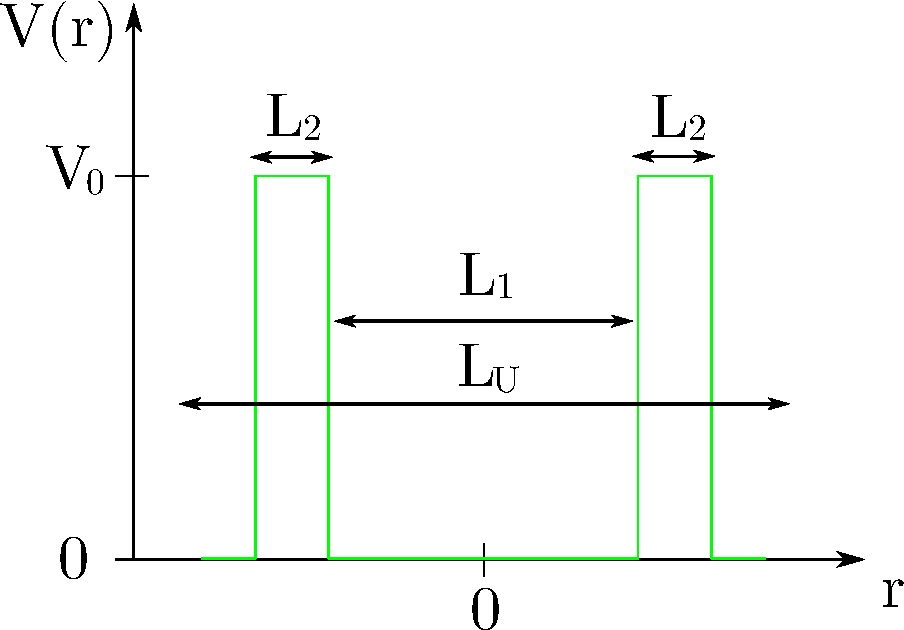
\includegraphics[width=0.7\textwidth]{plots/potential.pdf}
  \caption{Potentialverlauf der RTD.}
  \label{fig:pot1}
\end{figure}
Die eingezeichneten Längen wählen wir wie in \cite{lukas1} zu
\begin{align}
  L_1 &= \SI{6}{\nano\meter}\\
  L_2 &= \SI{5}{\nano\meter}\\
  L_U &= \SI{30}{\nano\meter} \; .
\end{align}
Hierin ist $L_U$ die Länge, über der die Spannung $U$ abfällt.



\section{Wigner Funktion}
\label{sec:wignerfunktion}
Es ist mit $\bra{x}\ket{\Psi} = \Psi(x)$
\begin{equation}
  P(x,p) \equiv \frac{1}{\pi\hbar} \int_{-\infty}^{\infty} \bra{x+y}\hat{\rho} \ket{x-y} \E{2ipy/\hbar} \diff y
\end{equation}
die Wigner-Funktion gleich der Wigner-transformierten des Dichteoperators $\hat{\rho}$. Die Wigner Transformation ist eine invertierbare Abbildung
\begin{align}
  W\; :\; L(\HR,\HR)  \rightarrow & \text{Phasenraum}^* \\
   \hat{G} \mapsto & g(x,p) = \int_{-\infty}^{\infty} \bra{x-s/2}\hat{G} \ket{x+s/2} \E{ips/\hbar} \diff s
\end{align}

\chapter{DG Verfahren}
\todo{konzeptionelle Beschreibung des Verfahrens, Vor- und Nachteile gegenüber anderen Verfahren / Motivation. Numerischer Fluss in Anlehnung an den Fluss im FV Verfahren ...}
\section{Konsistenz (in Anlehnung an den Vortrag)}
\label{sec:konsistenz}
Unter Konsistenz verstehen wir, dass die Lösung der pDGL auch die von uns gewählte variationale Formulierung erfüllt.
\begin{itemize}
  \item
Dies bedeutet in Sichtweise A (numerischer Fluss)
\begin{align}
  f^*(u,u) = f(u)
\end{align}
Hierbei ist $f(u)$ der Fluss, der den Teil nach partieller Integration beschreibt.
\begin{align}
  \int_{K} v\operatorname{div}(A\nabla u) = \int_K \nabla v \cdot \underbrace{(-A\nabla u)}_{\equiv f(u)} + \int_{\partial K} v A\nabla u \cdot n_K
\end{align}
Hingegen ist $f^*(u^+,u^-)$ der numerische Fluss, der anhand der Charakteristik der pDGL gewählt werden kann. Diese Wahl ist das Herzstück der DG-Methoden. Die Wahl sollte Stabilität und Konsistenz gewährleisten. Stabilität bedeutet hier, kleine Änderungen der Daten resultieren in kleinen Änderungen der (numerischen) Lösungen. Außerdem auch, dass die Zeitableitung beschränkt ist, genauer gesagt
\begin{align}
  \sum_{K=1}^{\#\mathcal{T}}\td{}{t}\norm{u_N}^2_{2;K} \leq 0
\end{align}
\item
In Sichtweise B (Bilinearform) bedeutet Konsistenz erneut, dass die Lösung der pDGL die von uns gewählte variationale Formulierung, sprich die Galerkin-Gleichung, erfüllt.
\begin{align}
  \mathcal{B}_N(u,V) = F_N(V) \qquad \forall \, {V\in\mathbb{V}_N}
\end{align}
Wir können in unserer Bilinearform beliebig Sprünge ergänzen, denn für die exakte Lösung gilt Stetigkeit und daher $\llbracket u \rrbracket = 0$.
\end{itemize}


% \section{Vortrag}
% \begin{align*}
%   q \longrightarrow k \\
%   \rho|_{q=\pm L_q/2} = ?\\
%   \rho|_{r=\pm L_r/2} = \hat{f}_{l,r}(q) \\
%   f(r,k) \\
%   \hat{\rho}(r,k) = \Phi \rho(r,q) \\
%   \rho(r,k>0)|_{r=- L_r/2} = \Phi \hat{f}_{l}(q) \\
%   \rho(r,k<0)|_{r=+ L_r/2} = \Phi \hat{f}_{r}(q) \\
%   f(r,k>0)|_{r=- L_r/2} = f_{l}(k) \\
%   f(r,k<0)|_{r=+ L_r/2} = f_{r}(k) \\
%   u \in \mathbb{V} \\
%   \mathbb{V}_{\mathcal{T}} \\
%   u_h
% \end{align*}
%
% \begin{align*}
%   E:\, C^1(\bar{\Omega}) \rightarrow \mathbb{R} \\
%   \td{}{\epsilon}E(u+\epsilon v) = 0 \\
%   E(u) = \frac{\sigma}{2} \int_{\Omega}|\nabla u|^2 - \int_{\Omega} fu \\
%   \int_{\Omega} \nabla u \cdot \nabla v = \int_{\Omega} fv \qquad \forall v\in\mathbb{V}_0\\
%   \mathcal{B}(u,v) = \int_{\Omega} \nabla u \cdot \nabla v \qquad f(v) \equiv (f,v)_{L^2(\Omega)} \\
%   \mathcal{B}(u,v) = f(v)\\
%   u\in\mathbb{V}
% \end{align*}
% \begin{align*}
%   \mathbb{V}_N \subset \mathbb{V} \\
%   U_N \in \mathbb{V}_N \\
%   \mathcal{B}(U_N,V_N) = f(V_N) \qquad \forall V_N\in\mathbb{V}_N \\
%   \mathbb{V}_N \subset \mathbb{V} \; \Rightarrow \; \mathcal{B}(u - U_N,V_N) = 0 \\
%   \mathcal{B}(v,v) \geq \alpha \norm{v}_{\mathbb{V}}^2 \qquad \forall v\in\mathbb{V}\\
%   \mathcal{B}(u,v) \leq \norm{\mathcal{B}}\norm{u}_{\mathbb{V}}\norm{v}_{\mathbb{V}} \qquad \forall u,v\in\mathbb{V}\\
%   f\in\mathbb{V}^*
% \end{align*}
% \begin{align*}
%   \alpha\norm{U_N-u}_{\mathbb{V}}^2 &\leq \mathcal{B}(U_N-u,U_N-u) = \mathcal{B}(U_N-u,V-u) \\
%   &\leq\norm{\mathcal{B}}\norm{U_N-u}_{\mathbb{V}}\norm{V-u}_{\mathbb{V}} \qquad \forall V\in\mathbb{V}_N\\
%   \Rightarrow \;\; \norm{U_N-u}_{\mathbb{V}} \leq \frac{\norm{\mathcal{B}}}{\alpha}\inf_{V\in\mathbb{V}_N}\norm{V-u}_{\mathbb{V}}
% \end{align*}
% \begin{align*}
%   i \partial_t u + \operatorname{div}(A\nabla u) - Bu &= 0  \qquad &\forall \vb{x}\in\Omega \\
%   u &= u_D                  & \forall \vb{x}\in\Gamma_D \subset \partial\Omega \\
%   A\nabla u \vb{n} &= U_N   & \forall \vb{x}\in\Gamma_N \subset \partial\Omega\\
%   \int_{\Omega} i \partial_t u v + \operatorname{div}(A\nabla u) v - Buv = 0 \qquad \forall v \in \mathbb{V} \\
%   \int_{\Omega} i \partial_t u v - (A\nabla u)\cdot \nabla v - Buv + \int_{\partial\Omega}(A\nabla u)v\cdot n = 0 \qquad \forall v \in \mathbb{V} \\
% \end{align*}
%
% \begin{align}
%   \fes(\mathcal{T},\mathbb{P}_N,\mathbb{V}) \equiv \{ V\in\mathbb{V} \, | \, V_{|K} \in \mathbb{P}_N(K) \, \forall \, K\in\mathcal{T}\}
% \end{align}
%
% \begin{align*}
%   -\Delta u = f \qquad \mathrm{in }\, \Omega, \qquad u=0 \qquad \mathrm{auf }\; \partial\Omega \\
%   u \in \mathbb{V}:\qquad \int_{\Omega}\nabla u\cdot\nabla v = \int_{\Omega} fv\qquad \forall\, v\in\mathbb{V}_0 \\
%   s - \frac{d}{2} \geq l \qquad \Rightarrow \qquad H^s(\Omega) \hookrightarrow C^l(\bar{\Omega})
% \end{align*}
%
% \begin{align*}
%   \{V\in C(\bar{\Omega})\,|\, V_{|K} \in \mathbb{P}_N(K)\,\forall K\in\mathcal{T}\} = \mathrm{FES}(\mathcal{T},\mathbb{P}_N,H^1(\Omega)) \\
%   \mathbb{V}_N = \mathrm{FES}(\mathcal{T},\mathbb{P}_N,\mathbb{V}) \not\subset \mathbb{V} \\
%   \norm{U_N - u}_N \lesssim (1+\frac{\norm{\mathcal{B}_N}}{\alpha_N})\inf_{V\in\mathbb{V}_N}\norm{V-u}_N+\frac{1}{\alpha_N}\sup_{V\in\mathbb{V}_N}\frac{|\mathcal{B}_N(u,V)-F_N(V)|}{\norm{V}_N}\\
%   \mathcal{B}_N : \, \mathbb{V}_N + \mathbb{V} \,\times\,\mathbb{V}_N\rightarrow \mathbb{R}\\
%   U_N(x_i)
% \end{align*}
%
% \begin{align*}
%   \pd{u(x,t)}{t} + \pd{(au(x,t))}{x} = 0\;,\qquad x\in[0,\ell] = \Omega\\
%   u(x,0) = u_0(x)\\
%   u(0,t) = g(t) \qquad \mathrm{mit}\,a\geq 0
% \end{align*}
%
% \begin{empheq}[box=\widefbox]{align}
%   i \partial_t \rho(r,q,t)+\operatorname{div}(A\nabla \rho(r,q,t)) - B(r,q,t) \rho(r,q,t) = 0
% \end{empheq}
%
% The numerical flux is chosen to ensure that information in the problem travels in the direction of the characteristic curves of the equation (upwinding). As mentioned in the comments, the numerical flux is necessary in order to couple the subproblems defined on each element.
%
% One way to get an intuition for the role of the numerical flux is to consider the following simple example.
%
% Consider the scalar advection equation (where for simplicity $a=1$)
% $$
% \frac{\partial u}{\partial t} + \frac{\partial u}{\partial x} = 0 \qquad\text{on $\Omega$},
% $$
% where the domain is given by $\Omega = [0,1]$. Because this is a hyperbolic equation, and information is propagating from left to right, we need to enforce a boundary condition at $x = 0$ (but not at $x = 1$). For concreteness, suppose we enforce the Dirichlet condition $u(0,t) = g_D$ for some given $g_D$.
%
% Suppose now we discretize this equation using the DG method, and we use two elements, $D_1 = [0,1/2]$ and $D_2 = [1/2,1]$. We could equally-well be discretizing the following set of two coupled PDEs,
% \begin{align*}
% \text{(PDE 1):} && v_t + v_x &= 0 \quad\text{auf $D_1=[0,\ell/2]$},\\
% \text{(PDE 2):} && w_t + w_x &= 0 \quad\text{auf $D_2=[\ell/2,\ell]$},
% \end{align*}
% where we will couple these equations to make them equivalent to the original equation.
%
% To make the above equations well-posed, we need to enforce boundary conditions. As before, each equation is hyperbolic, and information is traveling from left to right. Therefore, we need to enforce a boundary condition for (PDE 1) on the left endpoint of $D_1$, and a boundary condition for (PDE 2) on the left endpoint of $D_2$.
%
% The boundary condition on the left endpoint of $D_1$ must be chosen to be $v(0,t) = g_D$ in order to remain consistent with the original problem. We also look for smooth solutions, so the boundary condition on the left endpoint of $D_2$ must be chosen to enforce continuity. This condition reads $w(1/2,t) = v(1/2,t)$.
%
% The DG method in this case chooses the numerical fluxes precisely to enforce the above boundary conditions. If we multiply by a test function $\psi$ and integrate by parts over each element $D_k$, we obtain boundary terms of the form
% \begin{align*}
%   \int_{D_1} \psi v_t - \int_{D_1} \psi_x \, v + \int_{\partial D_1} \psi  v \hat{n}  &= 0\\
%   \int_{D_1} \psi_N v_{N,t} - \int_{D_1} \psi_{N,x}  v_N + \int_{\partial D_1} \psi_N  \,v_N^* \, \hat{n}  &= 0 \\
% \int_{\partial D_1} \hat{n} \cdot v \psi \, dx &= \left[ v\psi \right]_0^{\ell/2}\\
% \int_{\partial D_2} \hat{n} \cdot w \psi \, dx &= \left[ w\psi\right]_{\ell/2}^\ell \\
% \end{align*}
% In order to "weakly" enforce the boundary conditions, we replace $v$ and $w$ with the prescribed values at those points where boundary conditions are specified (i.e. the left endpoints of $D_1$ and $D_2$). This means we replace $v(0,t)$ by $g_D$ and $w(1/2,t)$ by $v(1/2,t)$ in the boundary integrals.
%
% In other words, we define $u_h^* = g_D$ at $x = 0$, and $u_h^* = v(1/2,t)$ at $x=1/2$, and we recover exactly the standard upwind flux that is used in the DG method.
%
% Looking at things this way, we can consider the numerical flux functions as weakly enforcing the boundary conditions on each element that are required to couple the equations in such a way that respects the characteristic structure of the equations.
%
% For equations more complicated than constant-coefficient advection, information may not propagate always in the same direction, and so the numerical flux must be determined by solving (or approximating the solution to) a Riemann problem at the interface. This is discussed for linear problems in Section 2.4 of Hesthaven's book.
% \begin{align*}
%   v_N^* = v_N^* (v_N^-, v_N^+) = \left\{  \begin{array}{l l} g(t), \; &x = 0 \\ \avg{v_N} + \frac{1}{2}\jump{v_N} = v_N^-(\ell/2, t) ,\; &x=\ell/2 \\ v_N^+(\ell,t),\; &x=\ell\end{array}  \right.
% \end{align*}
% \begin{align*}
%   \Leftrightarrow \qquad f^*(u,u) = f(u)\\
%   u \in H^1(\Omega)
% \end{align*}

\section{DG Schema}
Wir verwenden das sogenannte \emph{local} DG (LDG) Verfahren \cite{cockburnLDG} und schreiben dazu die Differentialgleichung zweiter Ordnung in ein System von Differentialgleichungen erster Ordnung um.
\begin{align}
  i \partial_t u(x,y,t)+\operatorname{div}(\underbrace{A\nabla u(x,y,t)}_{\equiv \vb{q}}) - \underbrace{ B(x,y,t) u(x,y,t)}_{\equiv g(u)} = 0 \\
  \left\{ \begin{array}{c}  i \partial_t u+\operatorname{div}( \vb{q}) - g(u) = 0 \\  \frac{1}{2}\partial_y u =  q_x \\ \frac{1}{2}\partial_x u =  q_y  \end{array}\right.
  \label{eq:gls1}
\end{align}
Als Ansatzraum wählen wir wie üblich den endlichdimensionalen Funktionenraum der stückweisen, zweidimensionalen Polynome vom Grad $N_p-1$.
\begin{equation}
  \mathbb{V}_N = \bigoplus\limits_{K\in\mathcal{T}}^{} \{\Psi_n(K)\}_{n=1}^{N_p}
\end{equation}
Hierbei ist $\mathcal{T}$ die Triangulierung des Rechengebietes, sodass mit $K$ eine einzelne Zelle bezeichnet wird. Für eine optimale Konditionierung der weiter unten eingeführten Massenmatrix ist es gemäß \cite{buch} sinnvoll, die orthonormierte Basis
\begin{equation}
  \Psi_m(x,y) = \sqrt{2}P_i(a)P_j^{(2i+1,0)}(b)(1-b)^i
\end{equation}
mit
\begin{align}
  a = 2\frac{1+x}{1-y} \qquad b = y
\end{align}
zu wählen. Hierbei bezeichnet $P_n^{(\alpha,\beta)}$ das Jacobi-Polynom. Die in dem Raum $\mathbb{V}_N$ liegende schwache Lösung ist durch eine Linearkombination der Basisfunktionen auf jeder Zelle $K$ der Triangulierung $\mathcal{T}$ eindeutig definiert.
\begin{align}
  \vb{x}\in K: \; u_N^K(\vb{x}) = \sum_{m=1}^{N_p}\hat{u}_N^K(t) \Psi_m(\vb{x})
  = \sum_{n=1}^{N_p} u_N^K(\vb{\xi}_n^K, t)\ell_n^K(\vb{x})
\end{align}
Die Darstellung links heißt "modale Entwicklung" und rechts "nodale Entwicklung", da hier die Entwicklungskoeffizienten wegen der Interpolationseigenschaft $\ell_n^K(\vb{\xi}_m^K)=\delta_{nm}$ gleich den Funktionswerten an den jeweiligen Interpolationspunkten $\vb{\xi}_n^K$ sind.
Abkürzend definieren wir
\begin{align}
  \underline{u}_N^K \equiv (u_N^K(\vb{\xi}_1^K, t),\dots, u_N^K(\vb{\xi}_{N_p}^K, t))^T \; .
\end{align}
Wir multiplizieren nun das Gleichungssystem \eqref{eq:gls1} mit der Testfunktion $\ell_i$, welche also ebenfalls Element des Ansatzraumes $\mathbb{V}_N$ ist. Ferner wird über die Zelle $K$ integriert und für den Divergenzterm eine partielle Integration durchgeführt. In unmittelbarer Anlehnung an das Schema für die Poissongleichung in zwei Dimensionen auf Seite 275, \cite{buch}, erhalten wir
\begin{align*}
  i\int_K \partial_t \sum_{j=1}^{N_p} u_N^K(\vb{\xi}_j^K, t)\ell_j^K(\vb{x}) \ell_i^K(\vb{x})
  - \int_K \sum_{j=1}^{N_p} \vb{q}_N^K(\vb{\xi}_j^K, t)\ell_j^K(\vb{x}) \cdot \nabla \ell_i^K(\vb{x}) \qquad \\
  \; + \int_{\partial K} \sum_{j=1}^{N_p} \vb{q}^{*,K}(\vb{\xi}_j^K, t)\ell_j^K(\vb{x}) \ell_i^K(\vb{x}) \cdot \hat{\vb{n}}
  - \int_K \sum_{j=1}^{N_p} g_N^K(\vb{\xi}_j^K, t)\ell_j^K(\vb{x}) \ell_i^K(\vb{x}) = 0 \\
  \forall i = 1,\dots,N_p
\end{align*}
\begin{align*}
  \int_K \sum_{j=1}^{N_p} u_N^K(\vb{\xi}_j^K) \partial_{\nicefrac{y}{x}} \ell_j^K(\vb{x})\ell_i^K(\vb{x}) + \int_{\partial K} \hat{n}_{\nicefrac{y}{x}} \sum_{j=1}^{N_p} (u^{*,K}(\vb{\xi}_j^K) -     u_N^K(\vb{\xi}_j^K))\ell_j(\vb{x})\\
   = 2 \int_K \sum_{j=1}^{N_p} (\vb{q}_N^K)_{\nicefrac{x}{y}} (\vb{\xi}_j^K, t) \ell_i^K(\vb{x})\ell_j^K(\vb{x})
\end{align*}
Wegen der nicht eindeutigen Definition der schwachen Lösung am Zellenrand (sie ist eben \emph{discontinuous}) müssen wir an dieser Stelle entscheiden, welchen Wert wir einsetzen wollen. Dazu erinnern wir uns an den vorangegangenen Abschnitt \ref{sec:konsistenz} und verwenden den numerischen Fluss $\vb{q}^{*,K}$ bzw. $u^{*,K}$, welchen wir später noch definieren müssen, um Konsistenz und Stabilität zu gewährleisten.

Definiere nun die Massenmatrix
\begin{align}
  (M^K)_{i,j} \equiv \int_K \ell_i^K(\vb{x})\ell_j^K(\vb{x}) = J^K \int_{\hat{K}}\ell_i(\vb{x}) \ell_j(\vb{x}) \equiv J^K M
\end{align}
sowie die Steifigkeitsmatrix
\begin{align}
  (S^K_{\nicefrac{x}{y}})_{i,j} \equiv \int_K \partial_{\nicefrac{x}{y}} \ell_j^K(\vb{x})\ell_i^K(\vb{x}) = (M^K D_{\nicefrac{x}{y}})_{i,j}
\end{align}

\rule{\textwidth}{0.4pt}
 Einschub: Die letzte Gleichheit folgt aus folgendem:

 Mit dem Zusammenhang zwischen nodaler Basis $\ell_i(\vb{x})$ und modaler Basis $\Psi_i(\vb{x})$ gemäß \cite{buch}, Seite 182
 \begin{equation}
   \ell_i = \sum_{j=1}^{N_p} (V^{T})^{-1}_{ij} \Psi_j
 \end{equation}
 und der logischen Tatsache, dass auch die Ableitung der modalen Basis (es handelt sich um ein Produkt von Lagrange-Polynomen, also letztlich ein Polynom vom Grad $N$) sich in selbiger entwickeln lassen gemäß
 \begin{equation}
   \partial_x \Psi_j(\vb{x}) = \sum_{m=1}^{N_p} a_{jm}\Psi_m(\vb{x})
 \end{equation}
 folgt
 \begin{align*}
   \sum_n \ell_n \partial_x \ell_j |_{r_n} &= \sum_{n,m,p} (V^{T})^{-1}_{nm} (V^{T})^{-1}_{jp}\Psi_m\partial \Psi_p |_{r_n} \\
    &= \sum_{n,m,p,q} (V^{-1})_{mn}(V^{T})^{-1}_{jp} \Psi_m a_{pq} V_{nq}\\
    &= \sum_{p,q}(V^{T})^{-1}_{jp}\Psi_q a_{pq} \\
    &= \sum_p (V^{T})^{-1}_{jp} \partial_x \Psi_p\\
    &= \partial_x \ell_j
 \end{align*}
 Daher gilt
 \begin{align}
   \int_K \partial_{\nicefrac{x}{y}} \ell_j(\vb{x})\ell_i(\vb{x}) &= \sum_n \int_K   \ell_n (\partial_{\nicefrac{x}{y}} \ell_j |_{r_n}) \ell_i \\
   &= \sum_n \underbrace{\partial_{\nicefrac{x}{y}} \ell_j |_{r_n}}_{\equiv (D_x)_{nj}} \int_K \ell_n \ell_i \\
   &= (M^K D_x)_{i,j}
 \end{align}
\rule{\textwidth}{0.4pt}

Einsetzen der soeben definierten Matrizen liefert
\begin{align}
  iM^K\partial_t \underline{u}_N^K - (S^K_x)^T (\underline{\vb{q}}_N^K)_x - (S^K_y)^T (\underline{\vb{q}}_N^K)_y
  + \int_{\partial K}  \hat{\vb{n}} \cdot \underline{\vb{q}}^{*,K} \underline{\ell}^K(\vb{x}) \ell_i^K(\vb{x})
  - M^K\underline{g}_N^K = 0
\end{align}
\begin{align}
  S_y^K \underline{u}^K_N + \int_{\partial K} \hat{n}_{y}  (\underline{u}^{*,K} - \underline{u}_N^K)\underline{\ell}(\vb{x})
  = 2 M^K (\underline{\vb{q}}_N^K)_x \\
  S_x^K \underline{u}^K_N + \int_{\partial K} \hat{n}_{x}  (\underline{u}^{*,K} - \underline{u}_N^K)\underline{\ell}(\vb{x})
  = 2 M^K (\underline{\vb{q}}_N^K)_y
\end{align}
Als Flüsse wählen wir versuchsweise
\begin{align}
  \underline{u}^{*,K} = \avg{\underline{u_N^K}}\\
  \underline{\vb{q}}^{*,K} = \avg{\underline{\nabla u_N^K}} - \tau\jump{\underline{u_N^K}}
\end{align}
mit einem \emph{Strafparameter} $\tau$, welcher Sprünge in der Ableitung bestraft, siehe \cite{buch}, Seite 270.

\section{Rankine-Hugoniot-Bedingung}
Die Rankine-Hugoniot-Bedingung steht im Zusammenhang mit dem sogenannten Riemann-Problem
\begin{align}
  u(x,0) = \begin{cases} u^- , & x < 0 \\
                         u^+ , & x > 0
           \end{cases}
\end{align}
für die Advektions-Gleichung
\begin{equation}
  u_t + f_x(u) = 0
\end{equation}
mit dem Fluss $f(u(x)) = s u(x)$.
Genaueres erfahren wir im Buch von LeVeque sowie in den Kapiteln 2.4 und 6.6 des Hesthaven Buches. Die Bedingung lautet im skalaren Fall
\begin{equation}
  s(u^- - u^+) = (f^- - f^+) \; .
  \label{eq:rhc}
\end{equation}
Die Größe s ist dabei die Geschwindigkeit, mit der sich die Diskontinuität ausbreitet (\emph{shock speed}). Im allgemeineren Fall eines linearen Systems mit $f(u) = A u$ nehmen wir an, dass die Matrix $A$ reelle, disjunkte Eigenwerte $\lambda_1 < \lambda_2 < \dots < \lambda_m$ hat, das heißt $A$ ist diagonalisierbar gemäß
\begin{equation}
  A = R \Lambda R^{-1}
\end{equation}
mit $R=[r_1 \, r_2 \, \dots \, r_m]$ als Transformationsmatrix mit den zugehörigen Eigenvektoren. Die Eigenwertgleichung lautet
\begin{equation}
  Ar_p = \lambda_p r_p \qquad \forall \, p=1,\dots, m
  \label{eq:EWeq_A}
\end{equation}
In unserem Fall wird $A$ ein symmetrisches Spektrum besitzen und so ausgelegt sein, dass der Eigenwert 0 nicht enthalten ist.  Daher gilt mit geradzahligem $m$
\begin{align}
  \lambda_i < 0 \qquad \forall \, i=1,\dots,m/2 \\
  \lambda_i > 0 \qquad \forall \, i=m/2+1,\dots,m \; .
\end{align}
Zerlegen wir nun $u^-$ und $u^+$ in die Eigenwertbasis gemäß
\begin{equation}
  u^- = \sum_{p=1}^m \alpha_p r_p \qquad u^+ = \sum_{p=1}^m \beta_p r_p,
\end{equation}
so folgt mit $v = R^{-1}u$
\begin{align}
  v_p(x,0) = \begin{cases} \alpha_p & x < 0 \\
                          \beta_p & x > 0 \end{cases}
\end{align}
und wegen der Charakteristik der Advektionsgleichung
\begin{align}
  v_p(x,t) = \begin{cases} \alpha_p & x - \lambda_p t < 0 \\
                           \beta_p & x - \lambda_p t > 0
            \end{cases}
\end{align}
Bezeichnen wir mit $J(x,t)$ den größtmöglichen Index $p$, für den $x-\lambda_p t > 0$ gilt., so ist
\begin{align}
  u(x,t) = \sum_{p=1}^{J(x,t)} \beta_p r_p + \sum_{p={J(x,t)}+1}^m \alpha_p r_p
\end{align}
und insbesondere für $x=0$
\begin{align}
  u(0,t) = \sum_{p=1}^{m/2} \beta_p r_p + \sum_{p=m/2+1}^m \alpha_p r_p
\end{align}
\todo{Tortendiagramm Buch S.66}
Die Lösung ist konstant innerhalb der einzelnen Segmente. Entlang der $p$-ten Charakteristik springt die Lösung jedoch gemäß
\begin{equation}
  \jump{u_p} = (\beta_p - \alpha_p) r_p \; ,
  \label{eq:TortenJump}
\end{equation}
wie der Abbildung zu entnehmen ist. Hier sehen wir auch wieder die Rankine-Hugoniot-Bedingung analog zu Gleichung \eqref{eq:rhc}, denn es ist mit $f(u) = A u$
\begin{align}
  \jump{f}_p &= A\jump{u}_p\\
  &\stackrel{\eqref{eq:TortenJump}}{=} (\beta_p - \alpha_p) A r_p \\
  &\stackrel{\eqref{eq:EWeq_A}}{=}  (\beta_p - \alpha_p) \lambda_p r_p \\
  &= \lambda_p \jump{u}_p
\end{align}
Um nun den numerischen Fluss $u^*$ zu bestimmen, interessieren wir uns für den Ort $x=0$ und können daher, entweder von $u^-$ ausgehend die Sprünge nach rechts aufaddieren oder von $u^+$ ausgehend die Sprünge nach links. Folglich gilt
\begin{align}
  \label{eq:rhc_1}
  u^* &= u^- + \sum_{\lambda_p < 0} (\beta_p - \alpha_p)r_p = u^+ - \sum_{\lambda_p > 0} (\beta_p - \alpha_p)r_p \\
  \Rightarrow \qquad u^* &= \frac{u^- + u^+}{2} + \frac{1}{2}\left( \sum_{\lambda_p < 0} (\beta_p - \alpha_p)r_p - \sum_{\lambda_p > 0} (\beta_p - \alpha_p)r_p \right)
\end{align}
Multipliziere mit $A=R\Lambda R^{-1} = R(\Lambda^+ + \Lambda^-)R^{-1}$
\begin{align*}
  (Au)^* = A \avg{u} + \frac{1}{2}& (R(\Lambda^+ + \Lambda^-)R^{-1}) \sum_{\lambda_p < 0} (\beta_p - \alpha_p)r_p \\
                     - \frac{1}{2}& (R(\Lambda^+ + \Lambda^-)R^{-1}) \sum_{\lambda_p > 0} (\beta_p - \alpha_p)r_p \\
         = A \avg{u} + \frac{1}{2}&\left( R\Lambda^-R^{-1} \sum_{\lambda_p < 0} (\beta_p - \alpha_p)r_p
                    - R\Lambda^+R^{-1} \sum_{\lambda_p > 0} (\beta_p - \alpha_p)r_p        \right)
\end{align*}
wegen $\sum_j (R^{-1})_{i,j} r_p = \delta_{i,p} e_p$ (mit $e_p$ als Einheitsvektor mit einer 1 an Stelle $p$). Fassen wir weiter zusammen:
\begin{align}
  (Au)^* &= A \avg{u} + \frac{1}{2} \left( -R|\Lambda^-|R^{-1} \sum_{\lambda_p < 0} (\beta_p - \alpha_p)r_p
              - R\Lambda^+R^{-1} \sum_{\lambda_p > 0} (\beta_p - \alpha_p)r_p        \right) \\
        &= A \avg{u} - \frac{1}{2} \underbrace{(R|\Lambda^-|R^{-1} + R\Lambda^+R^{-1})}_{=R|\Lambda|R \equiv |A|}  \sum_p(\beta_p - \alpha_p)r_p   \\
        &\stackrel{\eqref{eq:rhc_1}}{=} A \avg{u} - \frac{1}{2} |A| (u^+-u^-) \\
        &= A \avg{u} + \frac{1}{2} |A| \jump{u}
\end{align}
